\documentclass[11pt,a4paper]{article}
\usepackage[french]{babel}
\selectlanguage{french}
\usepackage[T1]{fontenc}
\usepackage[utf8]{inputenc}
\usepackage[left=2.00cm, right=2.00cm, top=2.00cm, bottom=1.80cm]{geometry}
\usepackage{enumitem}
\usepackage{siunitx}
\usepackage{graphicx}
\usepackage{titling}
\usepackage{textcomp}
\usepackage{comment} 
\usepackage{multicol}
\usepackage{caption}
\usepackage{xcolor} 
\usepackage{booktabs}
\usepackage{booktabs}
\usepackage{minted}
\usepackage[dvipsnames]{xcolor}
\usepackage{fancyvrb}
\usemintedstyle{autumn}
% permet le format paysage
\usepackage{lscape}
\usepackage{geometry}
\geometry{hmargin=3cm,vmargin=2cm}

\usepackage[compatibility=false, labelfont=bf]{caption} % justification=centering,
    \renewcommand\listingscaption{ }

% redefine \VerbatimInput
\RecustomVerbatimCommand{\VerbatimInput}{VerbatimInput}%
{fontsize=\footnotesize,
 %
 frame=lines,  % top and bottom rule only
 framesep=2em, % separation between frame and text
 rulecolor=\color{Gray},
 %
 label=\fbox{\color{Black}Sortie de la requête select * from resume\_table\_et\_vue },
 labelposition=topline,
 %
 commandchars=\|\(\), % escape character and argument delimiters for
                      % commands within the verbatim
 commentchar=*        % comment character
}



\begin{document}
%https://www.overleaf.com/7674422171kmqkcydhmxgs
\begin{titlepage}
    \centering
	
\includegraphics[width=0.25\textwidth]{img/logo.png}
	\par\vspace{1cm}
	\vspace{1cm}
	{\scshape\Large Compte-rendu de projet \\ Mégadonnées \par}
	\vspace{0.5cm}
	{\scshape\large Master 2 Bioinformatique pour les Biologistes\par}
	\vspace{1.5cm}
	{\LARGE\bfseries Travaux pratiques de bases de données\par}
	\vspace{2cm}
	{\Large Tanguy Lallemand, \\
            Jonathan Cruard, \\
            François Courtin, \\
            Louison Fresnais\par}
	\vfill

% Bottom of the page
    {\scshape\Large Université de Nantes \par}
    \vspace{1.5cm}
	{\large Année 2018/2019 \par}
\end{titlepage}

\newpage
\tableofcontents
\newpage

\section{Introduction}
    \paragraph{}
    Le but du projet est de concevoir une base de données Oracle (version 11g) permettant la gestion d'une bibliothèque. Cette base de données doit être capable de gérer les abonnés à la bibliothèque, les ouvrages présents ainsi que les emprunts réalisés par les abonnés.
    \par
    Un ouvrage sera identifié par un ISBN, un genre littéraire, un titre, un auteur ainsi qu'un éditeur. Chaque ouvrage peut être disponible en plusieurs exemplaires. Une table exemplaire est donc construite.
    \par
    Cette table exemplaire va stocker l'ISBN, un numéro d'exemplaire, l'état de l'ouvrage, le nombre de fois où l'exemplaire a été emprunté et la date à laquelle le nombre d'emprunts a été calculé pour la dernière fois.
    \par
    De même, les membres sont identifiés selon un ID unique d'adhérent mais aussi leurs nom et prénom et pour finir, leur adresse ainsi que leur numéro de téléphone. Les membres sont abonnés à la bibliothèque, c'est pourquoi, la date d'adhésion ainsi que la durée d'adhésion doivent aussi être stockées.
    \par
    Pour finir, la base de données devra aussi gérer les emprunts d'ouvrages. Dans cette optique, pour chaque emprunt, seront stockés: un ID d'emprunt unique, le membre qui est lié à cet emprunt ainsi que la date où il a été effectué. Pour chaque emprunt, seront aussi stockés les détails de celui-ci c'est-à-dire, l'exemplaire de l'ouvrage emprunté, la date de rendu. 
    Enfin, pour un numéro d'emprunt spécifique, on spécifie à quel membre il est attribué et à quelle date il a été réalisé. Le détail de cet emprunt indique quels exemplaires ont été empruntés. Ils sont identifiés par un numéro d'ouvrage, par numéro d'emprunt et il est indiqué la date à laquelle ils ont été rendus et par quel employé le retour du livre a été fait.\\
    \par
    L'ensemble de ces informations sont résumées dans la figure suivante (figure \ref{fig:diag}). Ce diagramme entité association rassemble les différentes tables de la base de données, les différents attributs ainsi que leur type associé. Les clés primaires permettant de faire le lien entre les tables sont soulignées. Les cardinalitées régissant les liens entre les tables sont aussi présentes dans ce diagramme.
\begin{landscape}
    \begin{figure}[h]
        \centering
        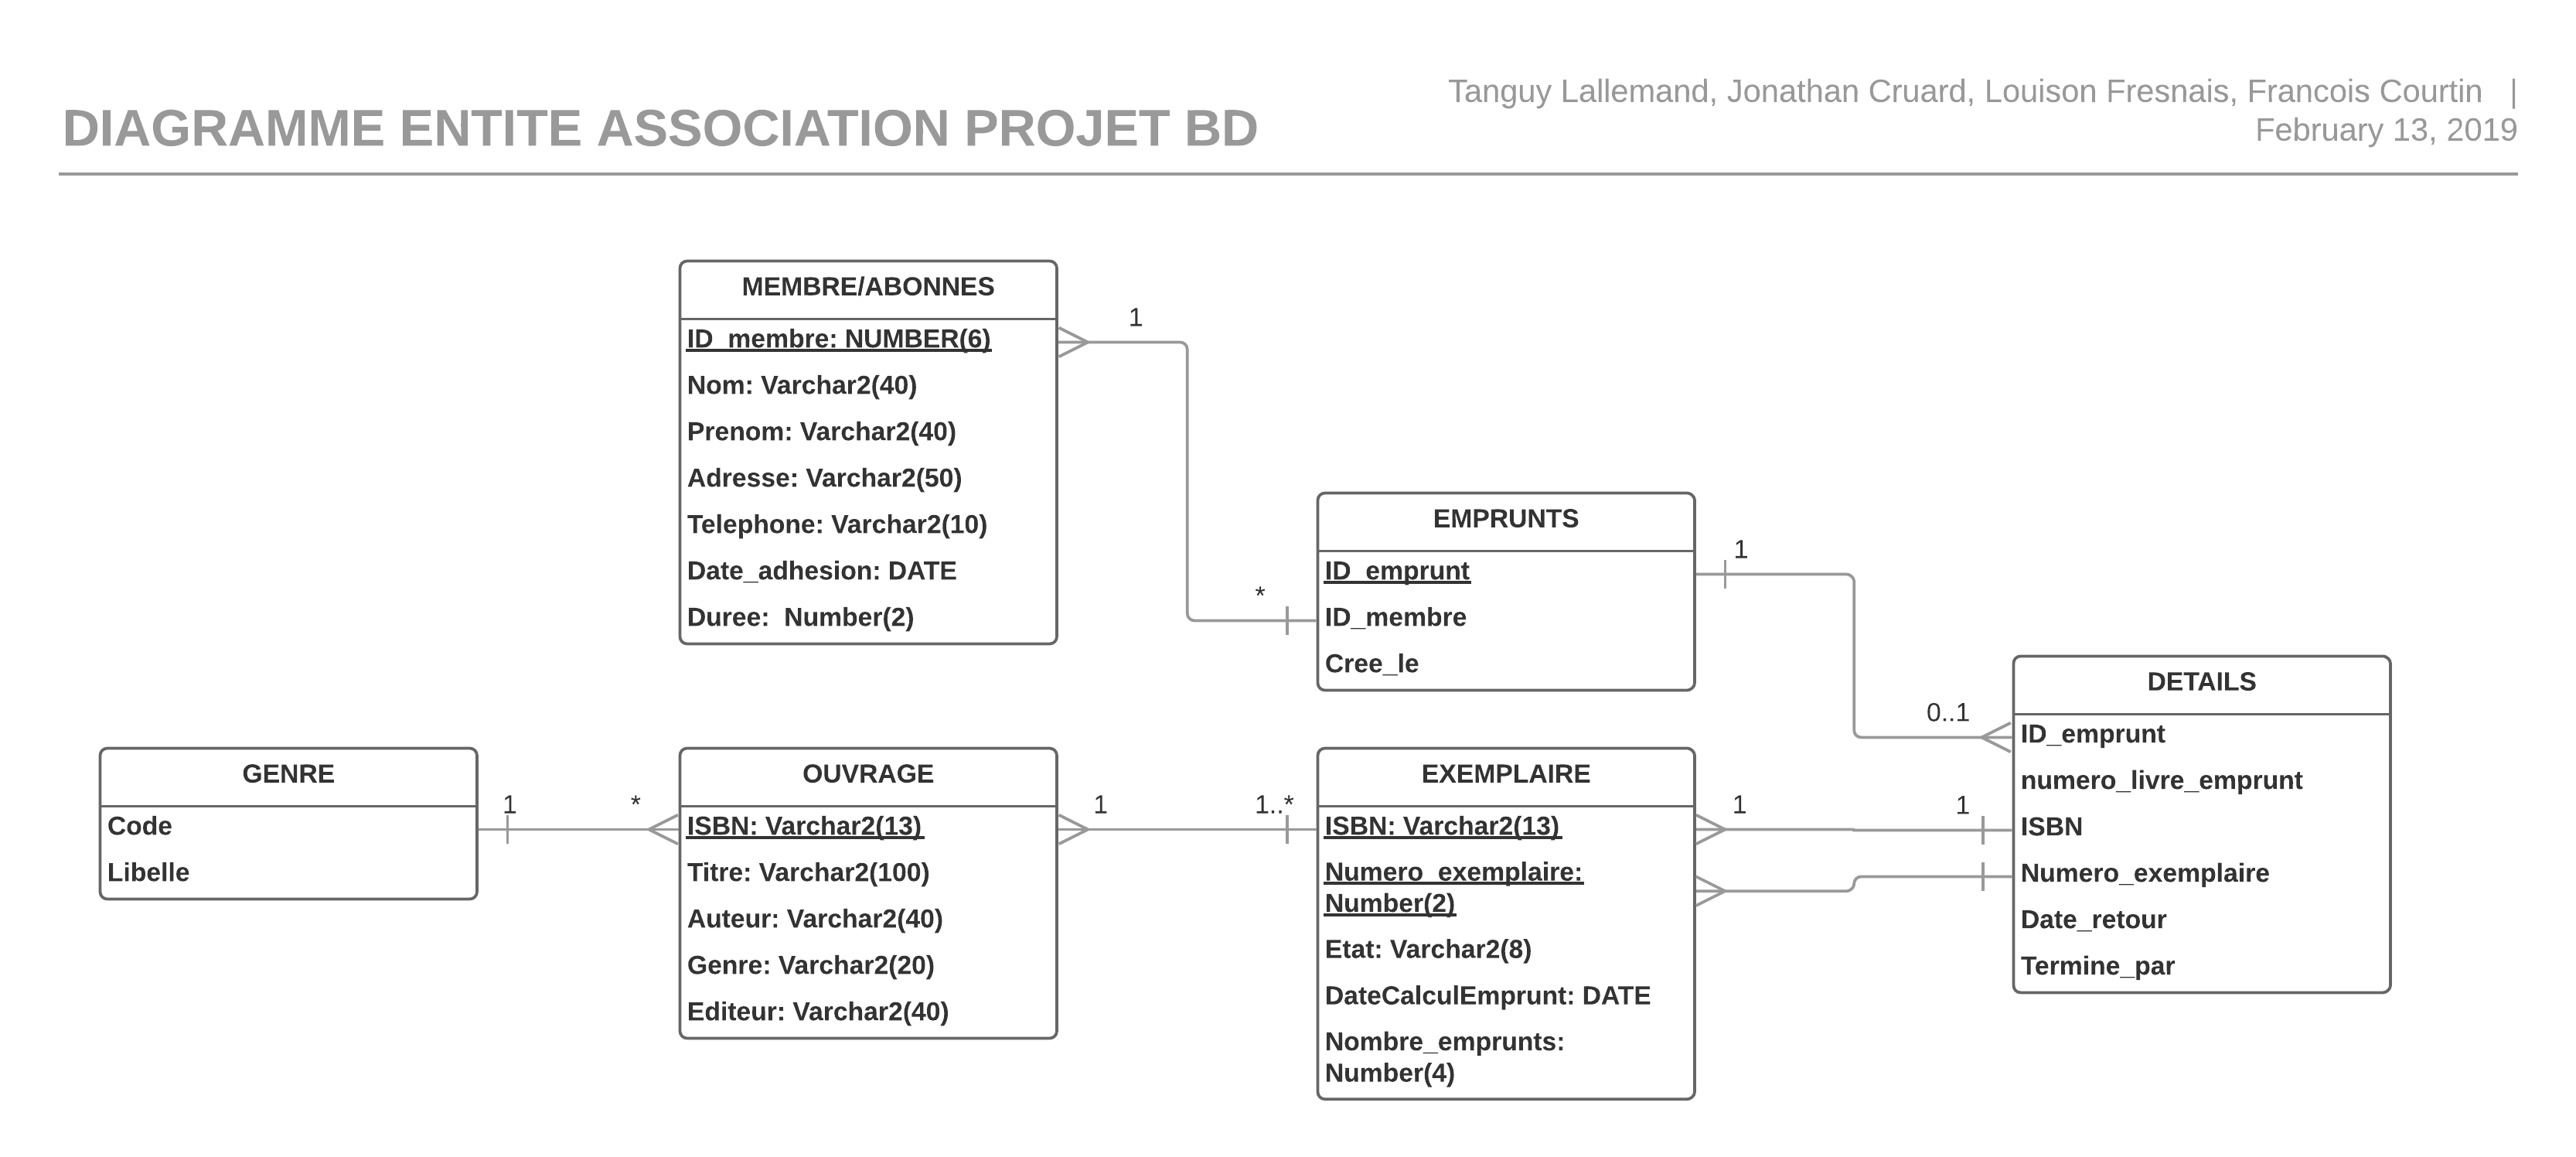
\includegraphics[width=26cm]{img/Diagramme_entite_association_db.png}
        \caption{Diagramme entité association}
        \label{fig:diag}
    \end{figure}
\end{landscape}
Les fonctionnalités implémentées autour de la base de données sont organisées en différents \textit{packages} regroupant toutes les fonctionnalités du même type. Un fichier contient également l'ensemble des \textit{triggers} de la base de données. De plus, les différentes requêtes permettant d'accéder aux données stockées dans la base sont stockées dans des \textit{views}.
\section{Fonctionnalités implémentées}
\subsection{SQL}
Les tables sont construites en SQL avec l'ensemble des colonnes nécessaires au bon fonctionnement de la base dans le temps. De plus, le type utilisé pour définir chaque colonne est adapté et optimisé afin d'économiser au maximum la mémoire. Des contraintes sont également définies pour garantir quand cela est nécessaire l'intégrité des informations stockées dans la base de données.
Ces contraintes sont des types suivant :
\begin{itemize}
    \item Clés primaires et secondaires
    \item Impossibilité pour une colonne de contenir la valeur 'NULL'
    \item Impossibilité de créer des enregistrements contenant la même combinaison de valeurs qu'un autre déjà existant (exemple : nom, prénom, numéro de téléphone)
    \item Obligation que les valeurs contenues dans la colonne appartiennent à une liste prédéfinie
    \item Obligation pour les valeurs d'une colonne de respecter une expression régulière
\end{itemize}
\par
Dans le but de garantir l'intégrité des clés primaires utilisées dans la base de données des séquences sont mises en place. Ces séquences vont fournir un numéro qui n'a pas été attribué lorsqu'elles sont appelées pour créer une nouvelle entrée dans la base de données évitant ainsi que l'utilisateur n'essaie pas d'attribuer un identifiant déjà utilisé.
\par
Un certain nombre de vues ont également été crées. Celles-ci fonctionnent comme des raccourcis permettant d'exécuter des requêtes de sélection prédéfinies. Ce qui permet à l'utilisateur d'accéder rapidement à des informations générales sur la base de données sans avoir à écrire de requête. Le fait d'intégrer des vues a plusieurs avantages. Tout d'abord, cela permet de cacher la complexité ce qui peut être un avantage dans le cas d'utilisateurs peu expérimentés en SQL, ce qui peut être le cas pour des employés de bibliothèque pas forcément formés en SQL. Les vues permettent aussi d'augmenter la sécurité de la base de donnée puisque une vue peut sélectionner certaines colonnes et/ou lignes d'une table, et il est possible à l'administrateur de la base de données de définir les permissions sur la vue au lieu des tables sous-jacentes. Cela permet de ne faire apparaître que les données qu'un utilisateur a besoin/le droit de voir. Pour finir, les vues peuvent simplifier la prise en charge du code existant. En effet, si vous avez besoin de changer une table ce qui rendrait obsolète beaucoup de code, il est alors possible de remplacer la table par une vue du même nom. La vue fournit exactement le même schéma que la table d'origine, alors que le schéma réel a changé. Ainsi, l'ancien code qui fait référence à la table ne se brise pas, ce qui vous permet de changer l'ancien code à votre guise.
Ainsi, l'ensemble des requêtes du projet ont été intégrées dans des \textit{views}. Dans un soucis de simplification, une vue appelée \textbf{resume\_table\_et\_vue} permet d'afficher l'ensemble des vues existantes. La figure suivante (\ref{vues} présente le résumé de la sortie de cette vue. Ainsi, si un utilisateur ne connaît pas l'ensemble des vues existantes il lui suffit d'exécuter la requête suivante: \textbf{SELECT * FROM resume\_table\_et\_vue}.


\begin{table}[h!]
    \centering
    \begin{tabular}{@{}l|l|@{}}
    \toprule
    TABLE\_NAME & TABLE\_TYPE \\ \midrule
    \multicolumn{1}{|l|}{ABONDANCE\_OUVRAGES} & VIEW \\
    \multicolumn{1}{|l|}{AFFICHE\_LIVRES\_AVEC\_DE} & VIEW \\
    \multicolumn{1}{|l|}{AFFICHE\_LIVRES\_AVEC\_MER} & VIEW \\
    \multicolumn{1}{|l|}{LISTER\_OUVRAGES\_ET\_EXEMPLAIRES} & VIEW \\
    \multicolumn{1}{|l|}{LISTE\_DES\_OUVRAGES} & VIEW \\
    \multicolumn{1}{|l|}{MEMBRE\_ORDRE\_ALPHA} & VIEW \\
    \multicolumn{1}{|l|}{NBR\_EMPRUNT} & VIEW \\
    \multicolumn{1}{|l|}{NBR\_OUVRAGE} & VIEW \\
    \multicolumn{1}{|l|}{NBR\_OUVRAGE\_PAR\_GENRE} & VIEW \\
    \multicolumn{1}{|l|}{OUVRAGES\_PAR\_GENRE} & VIEW \\
    \multicolumn{1}{|l|}{OUVRAGE\_AVEC\_PUBLIC} & VIEW \\
    \multicolumn{1}{|l|}{OUVRAGE\_EMPRUNTE\_DEPUIS\_2\_SEM} & VIEW \\
    \multicolumn{1}{|l|}{OUVRAGE\_MOINS\_POPULAIRE\_3MOIS} & VIEW \\
    \multicolumn{1}{|l|}{OUVRAGE\_PLUS\_POPULAIRE\_12MOIS} & VIEW \\
    \multicolumn{1}{|l|}{OUVRAGE\_SANS\_NEUF} & VIEW \\
    \multicolumn{1}{|l|}{RESUME\_TABLE\_ET\_VUE} & VIEW \\
    \multicolumn{1}{|l|}{RESUME\_PROCEDURES\_ET\_FONCTIONS} & VIEW \\
    \multicolumn{1}{|l|}{TEMPS\_MOYEN\_EMPRUNT\_GENRE} & VIEW \\
    \multicolumn{1}{|l|}{TEMPS\_MOYEN\_EMPRUNT\_MEMBRE} & VIEW \\ \midrule
    \multicolumn{1}{|l|}{UNIQ\_ID\_EMPRUNT} & SEQUENCE \\
    \multicolumn{1}{|l|}{UNIQ\_ID\_MEMBRE} & SEQUENCE \\ \midrule
    \multicolumn{1}{|l|}{DETAILS} & TABLE \\
    \multicolumn{1}{|l|}{EMPRUNTS} & TABLE \\
    \multicolumn{1}{|l|}{EXEMPLAIRE} & TABLE \\
    \multicolumn{1}{|l|}{GENRE} & TABLE \\
    \multicolumn{1}{|l|}{MEMBRE} & TABLE \\
    \multicolumn{1}{|l|}{OUVRAGE} & TABLE \\ \bottomrule
    \end{tabular}
    \caption{Ensemble des vues accessibles et les tables associées à la base de données}
    \label{vues}
\end{table}


\par
Dans une problématique d'optimisation des requêtes, les jointures entre tables sont (dans la mesure du possible) évitées au profit de sous-requêtes, celles-ci étant moins coûteuses en ressources.

\subsection{PL/SQL}
Une partie du projet utilise le PL/SQL. Il permet dans certains cas de réaliser des opérations complexes que ne permet pas (ou pas facilement) SQL seul. De plus l'approche PL/SQL permet dans certains cas de rendre plus efficace la réalisation de l'opération voulue sur la base de données. Le PL/SQL a plusieurs avantages non négligeables dans la gestion de ce type de projet et notamment, la gestion de structures sous forme de bloc de code ce qui permet une maintenance plus facile du code. De plus ce langage apporte des constructions procédurales comme des variables, des conditions et des boucles ce qui permet d'écrire réutilisable dans plusieurs cas de figure qui pourrait être rencontrés au cours du projet. Pour finir, le PL/SQL permet d'augmenter la portablilité du code via la construction de fonctions mais aussi via la gestion des exceptions qui permet de produire un code moins sujet à des échecs d'exécution non gérées. C'est avec cette approche que nous avons cherché a implémenté la partie PL/SQL du projet. C'est pourquoi nous avons cherché a implémenté l'ensemble de cette partie sous forme de fonctions et procédures.

\subsubsection{Fonctions et procédures}
Afin d'optimiser la modularité de notre projet nous avons utilisé des \textit{packages} pour stocker nos fonctions et procédures cela permet de produire un code plus condensé et plus facile a lire et à maintenir. Un des avantages majeur des procédures et des fonctions est qu'il permet de séparer la partie de la logique d'accès aux données de la logique d'application. De plus en codant des fonctions suffisamment global il est possible d'écrire du code efficace et qui s'adapte a différents cas de figure. Par exemple, dans la partie III du projet, les questions 3 et 4 nous demandait de chercher a extraire des informations à l'aide de requêtes SQL et de \textit{regex}. Ces deux questions peuvent être solutionnées par la fonction \textbf{recherche\_pattern} que nous avons implémenté qui prend en argument un pattern \textit{regex} et va retourner les informations retrouvé à l'aide de ce pattern. Ainsi, cela permet donc de condensé le code et de le rendre le plus polyvalent possible.
Cela permet également leur encapsulation, facilitant l'organisation du code. Cela permet aussi de renforcé la sécurité de notre base de données et permettant notamment d'éviter les injections SQL puisque les entrées dans les fonctions sont contrôlées. De plus, cette encapsulation permet de pouvoir caché à l'utilisateur des sous-programmes permettant de ne dévoiler que le minimum à l'utilisateur.
Les \textit{packages} permettent aussi d'augmenter les performances de notre programme car lors de l'ajout des \textit{packages} les fonctions sont précompilées ce qui permet une vitesse d'exécution augmentée même si l'initialisation de la base de donnée est un peu moins rapide à cause de cette pré-compilation. Néanmoins, une fois chargé en mémoire, l'utilisation des fonctions ne requiert plus d'accès au disque ce qui, en plus de l'étape de compilation, permet une augmentation non négligeable des performances des fonctions. Cela permet aussi à certaines parties de notre code d'être ré-exploitables. Le seul inconvénient soulevé réside dans une petite perte d'optimisation de la mémoire, en effet toutes les fonctions doivent être chargées même lorsque l'on en utilise qu'une seule. Il faut également penser à recompiler tout le package à chaque modification d'une fonction ou d'une procédure à l'intérieur.
Ainsi dans un soucis de simplicité dans la prise en main de notre code les fonctions on été placées dans des \textit{packages} qui regroupent de façon logique les fonctions suivant leur rôle au sein du projet.
\par Ainsi nous avons créé un package de maintenance comportant des fonctions et procédures permettant de gérer l'état des emprunts ou encore la suppression des membres. Un package \textbf{infos} contenant des fonctions permettant d'obtenir des informations quant à l'activité de la base de données. Nous avons également un package \textbf{livre} regroupant les fonctions et procédures relatives aux ouvrages et aux emprunts.
\par
L'ensemble des procédures, fonctions et triggers accessibles par les utilisateurs sont affichables via une vue appelée resume\_procedures\_et\_fonctions. Le tableau \ref{fonctions} suivant résume la sortie de cette vue:

\begin{table}[h]
\centering
\begin{tabular}{lll}
\hline
\multicolumn{1}{|l|}{OBJECT\_NAME} & \multicolumn{1}{l|}{PROCEDURE\_NAME} & \multicolumn{1}{l|}{OBJECT\_TYPE} \\ \hline
\multicolumn{1}{|l|}{INFOS} & \multicolumn{1}{l|}{ANALYSEACTIVITE} & \multicolumn{1}{l|}{PACKAGE} \\
\multicolumn{1}{|l|}{INFOS} & \multicolumn{1}{l|}{ANALYSEACTIVITE\_DETAIL} & \multicolumn{1}{l|}{PACKAGE} \\
\multicolumn{1}{|l|}{INFOS} & \multicolumn{1}{l|}{ANALYSEACTIVITE\_EMPRUNT} & \multicolumn{1}{l|}{PACKAGE} \\
\multicolumn{1}{|l|}{INFOS} & \multicolumn{1}{l|}{LISTER\_OUVRAGES} & \multicolumn{1}{l|}{PACKAGE} \\
\multicolumn{1}{|l|}{INFOS} & \multicolumn{1}{l|}{RECHERCHE\_PATTERN} & \multicolumn{1}{l|}{PACKAGE} \\
\multicolumn{1}{|l|}{LIVRE} & \multicolumn{1}{l|}{ADHESIONAJOUR} & \multicolumn{1}{l|}{PACKAGE} \\
\multicolumn{1}{|l|}{LIVRE} & \multicolumn{1}{l|}{AJOUTEMEMBRE} & \multicolumn{1}{l|}{PACKAGE} \\
\multicolumn{1}{|l|}{LIVRE} & \multicolumn{1}{l|}{DUREEMOYENNE} & \multicolumn{1}{l|}{PACKAGE} \\
\multicolumn{1}{|l|}{LIVRE} & \multicolumn{1}{l|}{EMPRUNTEXPRESS} & \multicolumn{1}{l|}{PACKAGE} \\
\multicolumn{1}{|l|}{LIVRE} & \multicolumn{1}{l|}{EMPRUNTMOYEN} & \multicolumn{1}{l|}{PACKAGE} \\
\multicolumn{1}{|l|}{LIVRE} & \multicolumn{1}{l|}{FINVALIDITE} & \multicolumn{1}{l|}{PACKAGE} \\
\multicolumn{1}{|l|}{LIVRE} & \multicolumn{1}{l|}{MAJEETATEXEMPLAIRE} & \multicolumn{1}{l|}{PACKAGE} \\
\multicolumn{1}{|l|}{LIVRE} & \multicolumn{1}{l|}{MESUREACTIVITE} & \multicolumn{1}{l|}{PACKAGE} \\
\multicolumn{1}{|l|}{LIVRE} & \multicolumn{1}{l|}{RETOUREXEMPLAIRE} & \multicolumn{1}{l|}{PACKAGE} \\
\multicolumn{1}{|l|}{LIVRE} & \multicolumn{1}{l|}{SUPPRIMEEXEMPLAIRE} & \multicolumn{1}{l|}{PACKAGE} \\
\multicolumn{1}{|l|}{MAINTENANCE} & \multicolumn{1}{l|}{MAJ\_ETAT\_EMPRUNT} & \multicolumn{1}{l|}{PACKAGE} \\
\multicolumn{1}{|l|}{MAINTENANCE} & \multicolumn{1}{l|}{NUMBER\_USES\_BOOK} & \multicolumn{1}{l|}{PACKAGE} \\
\multicolumn{1}{|l|}{MAINTENANCE} & \multicolumn{1}{l|}{PURGEMEMBRES} & \multicolumn{1}{l|}{PACKAGE} \\
\multicolumn{1}{|l|}{CHECK\_EXPL} & \multicolumn{1}{l|}{-} & \multicolumn{1}{l|}{TRIGGER} \\
\multicolumn{1}{|l|}{INFOS} & \multicolumn{1}{l|}{-} & \multicolumn{1}{l|}{PACKAGE} \\
\multicolumn{1}{|l|}{INFO\_CREATE\_EMPRUNT} & \multicolumn{1}{l|}{-} & \multicolumn{1}{l|}{TRIGGER} \\
\multicolumn{1}{|l|}{INFO\_MODIF\_DETAILS} & \multicolumn{1}{l|}{-} & \multicolumn{1}{l|}{TRIGGER} \\
\multicolumn{1}{|l|}{LIVRE} & \multicolumn{1}{l|}{-} & \multicolumn{1}{l|}{PACKAGE} \\
\multicolumn{1}{|l|}{MAINTENANCE} & \multicolumn{1}{l|}{-} & \multicolumn{1}{l|}{PACKAGE} \\
\multicolumn{1}{|l|}{MAJ\_ETAT\_EXPLR} & \multicolumn{1}{l|}{-} & \multicolumn{1}{l|}{TRIGGER} \\
\multicolumn{1}{|l|}{MODIF\_MB\_EMPRUNT} & \multicolumn{1}{l|}{-} & \multicolumn{1}{l|}{TRIGGER} \\
\multicolumn{1}{|l|}{MOD\_REF\_EMPRUNT} & \multicolumn{1}{l|}{-} & \multicolumn{1}{l|}{TRIGGER} \\
\multicolumn{1}{|l|}{SUPPRIMER\_EXEMPLR\_MAUVAIS} & \multicolumn{1}{l|}{-} & \multicolumn{1}{l|}{TRIGGER} \\
\multicolumn{1}{|l|}{VALID\_EMPRUNT} & \multicolumn{1}{l|}{-} & \multicolumn{1}{l|}{TRIGGER} \\
VENR\_DETAIL & - & TRIGGER \\ \hline
\end{tabular}
\caption{Ensemble des procédures, fonctions et triggers accessibles associés à la base de données}
\label{fonctions}
\end{table}

\subsubsection{Triggers}
Les \textit{triggers} mis en place permettent principalement de mettre à jour les données "internes" à la base de données afin de tenir les informations à jour sans intervention d'un utilisateur.
Dans notre cas, il n'a pas toujours été possible d'utiliser les \textit{triggers} les plus optimaux (ex: mise à jour de tables spécifiques tous les jours après la fermeture de la bibliothèque) en raison de manque de droits.
Nous avons également tenté d'utiliser des jobs mais cela n'a pas non plus été possible (permissions).
Ceux-ci permettent également de bloquer des modifications de la base de données considérées comme "illégales" et donc de conserver l'intégrité des données.
\par
Cependant les \textit{triggers} possèdent quelques désavantages. En effet ils imposent un lourd chargement sur le serveur de la base de données. Ils ne sont également pas recommandés dans le cas de données changeant très rapidement en peu de temps, le serveur pourrait ne pas toujours supporter le nombre de déclenchements à la seconde.



\newpage

\section{Futures implémentations}
\subsection{Approche Objet relationnel}
Afin de chercher a améliorer le projet une approche possible pourrait être de réfléchir à une implémentation avec une approche objet relationnel. 
Pour se faire, il faut repenser les tables et les relations qui existent entre elles. Le schéma de la nouvelle base de données est fournis dans la figure suivante \ref{or}.
Ainsi, nous avons donc intégré à la table \textbf{EMPRUNTS} une colonne de type table \textbf{DETAILS} correspondant à l'emprunt. Cette table imbriquée permet de stocker plus logiquement les données structurées liées aux emprunts. 
La table \textbf{MEMBRE} inclus également une sous-table contenant des références vers les emprunts correspondants à ce membre. La table des \textbf{GENRE} à également été simplifiée et ne contient désormais plus que la colonne libellé à laquelle on fait référence dans la colonne genre de l'ouvrage.


\begin{landscape}
    \begin{figure}[h]
        \centering
        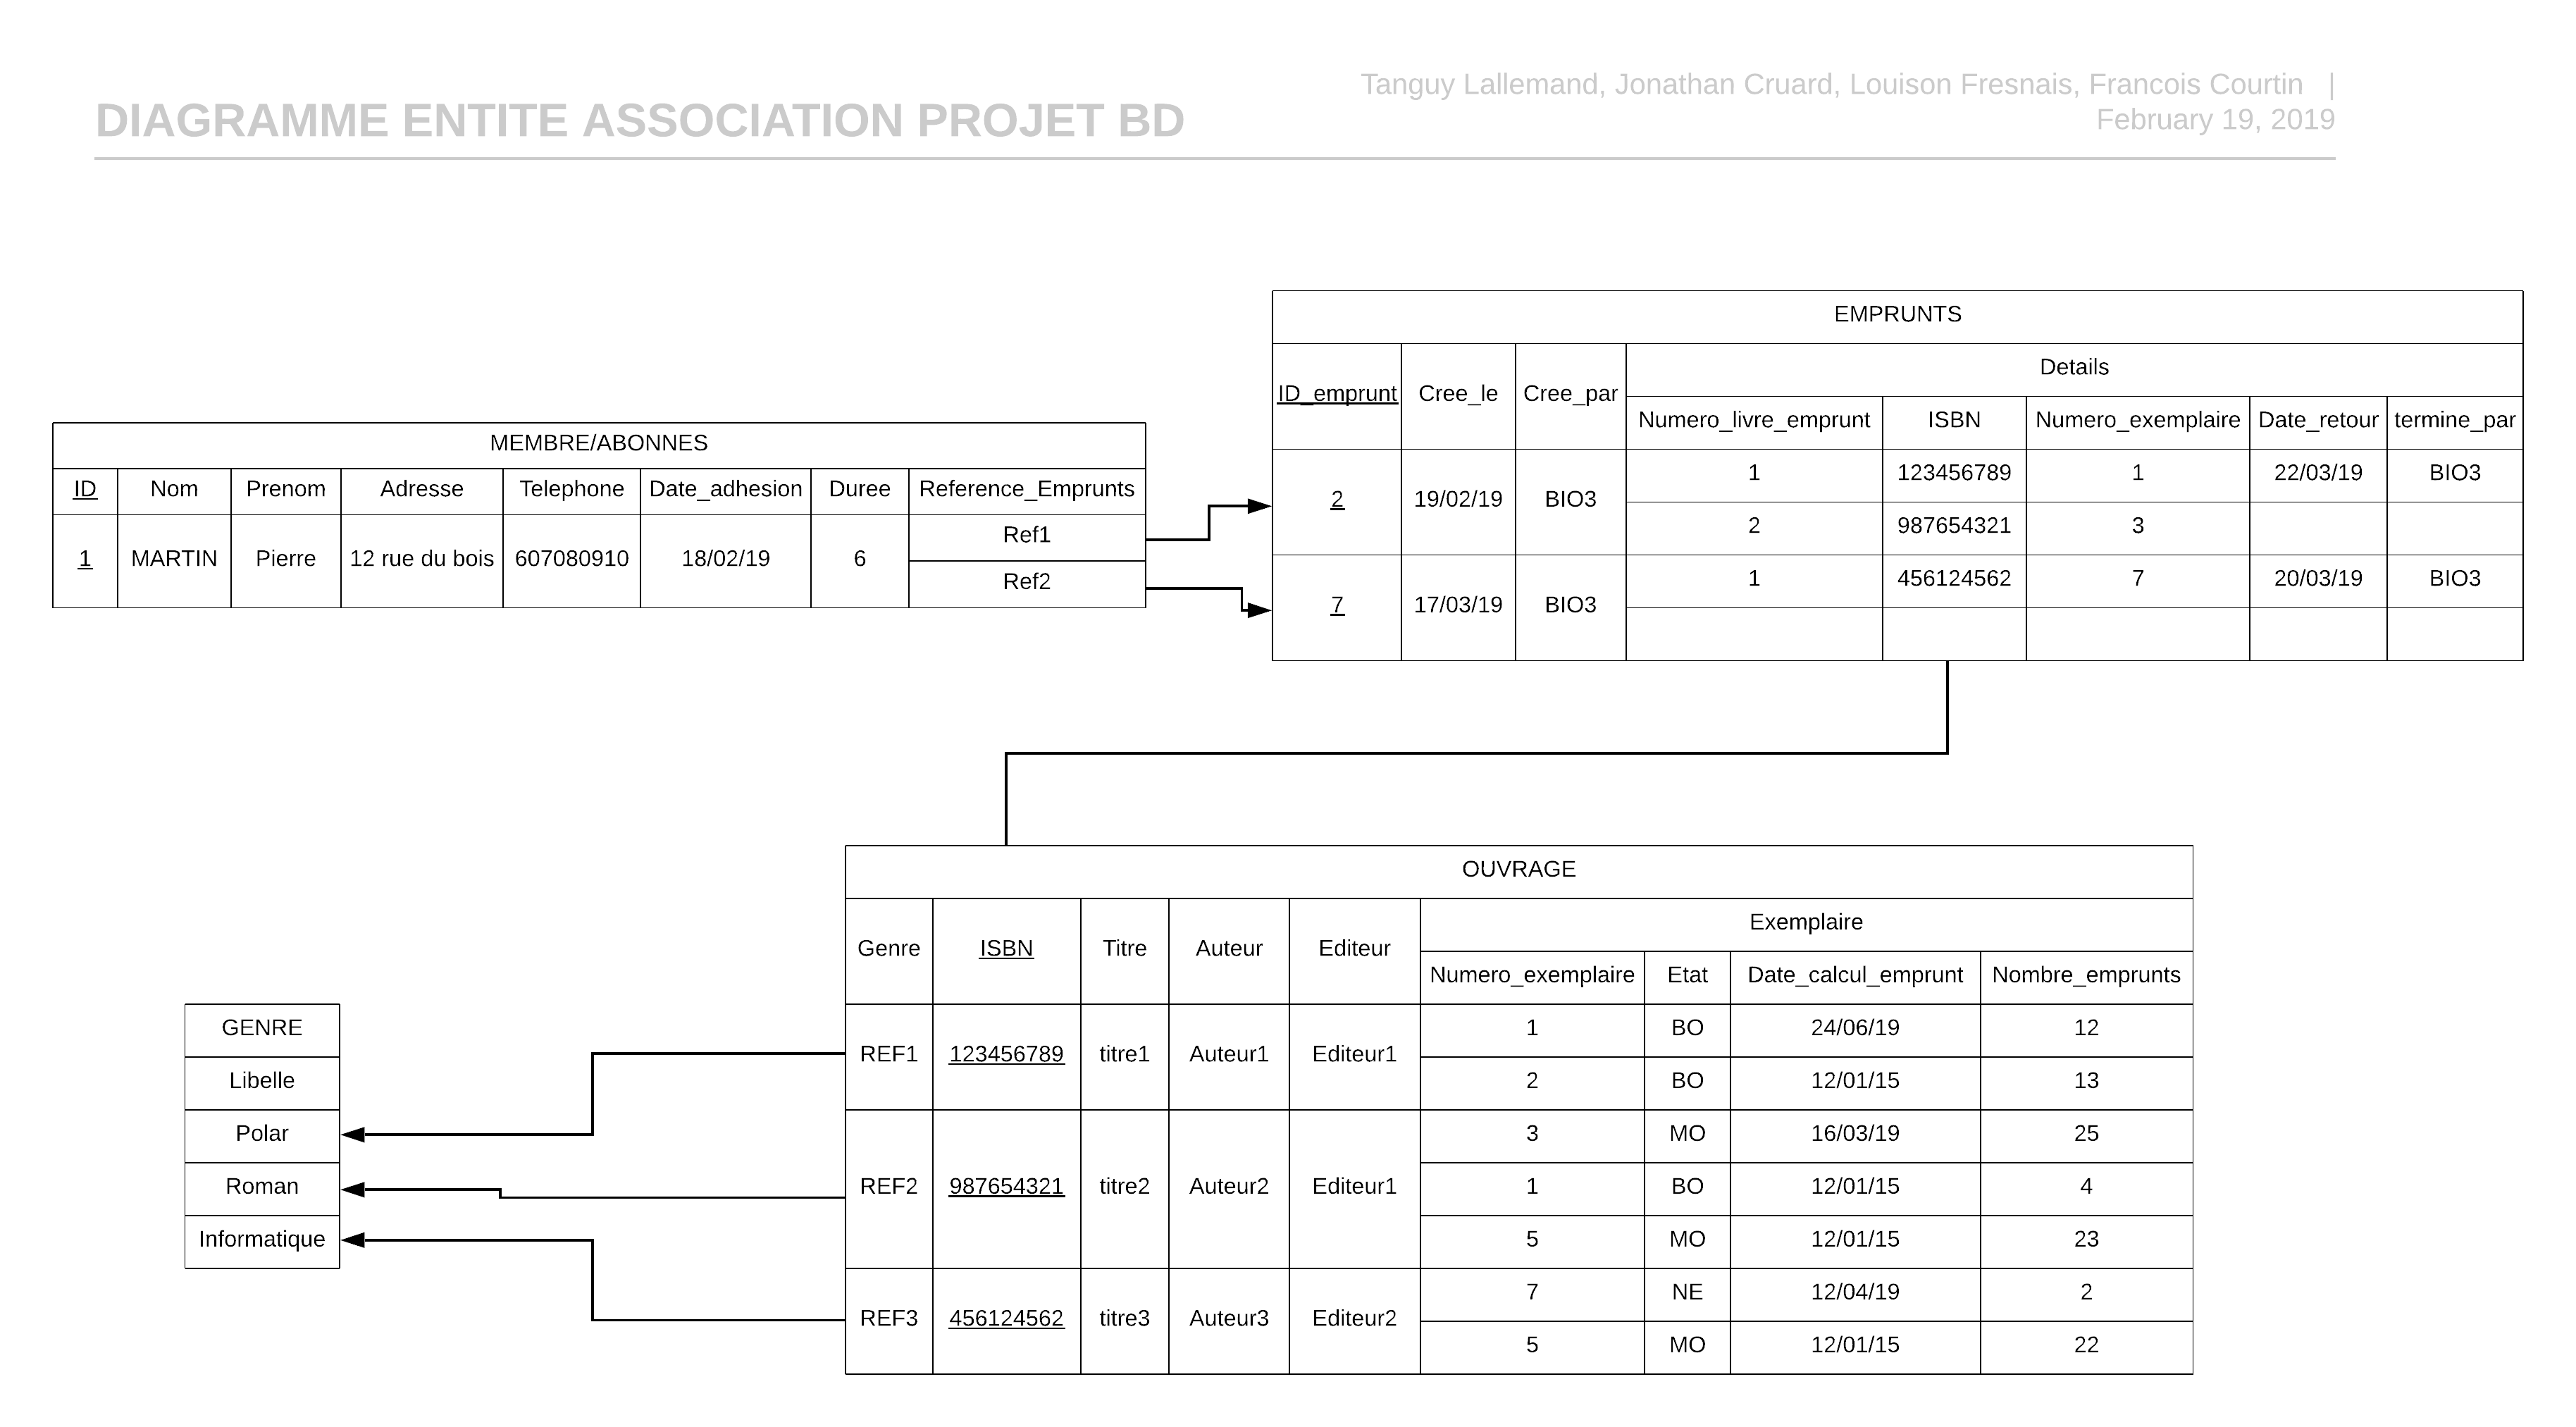
\includegraphics[width=26cm]{img/projet_megadonnees_v2.png}
        \caption{Schéma de la base de donnée suivant une approche objet relationnel}
        \label{or}
    \end{figure}
\end{landscape}

Cette approche avec des tables imbriquées a plusieurs avantages mais aussi un désavantages. Tout d'abord, la table imbriquée a l'avantage d'être indexée, et les groupes répétitifs sont séparés dans une autre table. Ceci permet de ne pas dégrader la performance des recherche dans la table complète. La table imbriquée permet également un nombre infini de groupes répétitifs. Cependant, il faut parfois plus de temps pour déréférencer l'OID pour accéder aux entrées de table imbriquées que les jointures de tables SQL ordinaires. De plus, à notre sens, si nous mettons de coté l'avantage pédagogique d'une telle implémentation, l'usage de table objet-relationnel serait limité pour une base de donnée de faible taille comme celle implémenté au cours du projet. En effet, la lecture 

\subsection{Implémentations annexes}
Pour améliorer le projet, il pourrait être intéressant de réfléchir à de nouvelles fonctions à ajouter afin de faciliter l'utilisation de la base de données. Il serait aussi intéressant, dans l'optique de garantir l'intégrité des données, d'ajouter d'autres \textit{triggers} afin de prévenir la survenue d'une éventuelle erreur de manipulation de la base de données.
\par
Afin d'étoffer la base de données il serait pertinent de répertorier des oeuvres numériques. Cela pourrait être fait par adaptation de la table ouvrages pour permettre l'ajout d'informations spécifiques à ce type d'oeuvre. Il faudrait par exemple modifier la colonne ISBN afin de permettre d'entrer des identifiants ISAN (l'équivalent de l'ISBN pour les oeuvres audiovisuelles), celui-ci est composé de 24 caractères en hexadécimal. Néanmoins si cette adaptation s'avère trop compliquée et que différentes colonnes supplémentaires sont nécessaires il sera alors nécessaire de créer une nouvelle table dédiée à ce type d'oeuvre.  
\par
Enfin un apport majeur à ce projet serait d'implémenter une interface graphique permettant d'interagir avec la base de données. On pourrait alors imaginer créer une table des "administrateurs" ou ajouter une colonne dans la table des membres afin de définir le niveau de droits qu'ils possèdent pour modifier la base de données. Ainsi il serait par exemple possible de permettre aux membres de consulter leurs emprunts en cours, la liste des ouvrages disponibles à l'emprunt, réserver un livre pour l'emprunter, etc.
Tandis que seuls les "administrateurs" seraient autorisés à enregistrer des données plus sensibles telles que la création d'un membre, un emprunt, un retour d'ouvrage, etc.
\section{Conclusion}
L'objectif principal du projet, à savoir la création d'une base de données répondant aux contraintes établies par le sujet à été rempli. Nous avons également réussi à ajouter des éléments permettant de sécuriser la base de donnée contre des erreurs internes ainsi que contre d'éventuelles injection SQL via les \textit{views} et les \textit{packages}.\\
Nous avons cherché à maximiser la modularité de notre code à l'aide de \textit{packages} contenant uniquement des fonctions et procédures permettant de réaliser un type d'action précis sur la base de donnée.
\textit{In fine}, la réalisation de ce projet nous a permis d'acquérir de nouvelles compétences en SQL et PL/SQL et notamment la nécessité de produire un code rigoureux pour le protégé d'erreurs ou d'attaques, mais également d'acquérir une vision plus globale de la gestion d'un projet de ce type notamment au niveau des améliorations annexes au projet.

\end{document}